\section{Compact Muon Solenoid}
\label{sec:Exp_CMS}
\subsection{Introduction}

%CMS has a broad program with goals of direct and indirect searches of BSM physics including supersymmetric particles as well as precision measurements of various SM parameters. 

% MAY NOT NEED THIS SENTENCE HERE
%Its main feature is a large magnet to create a magnetic field of~4T to curve charged particles in the tracking system and of~2T outside to curve muons in the muon system.

CMS is a general-purpose detector designed to register particles with energies of tens and hundreds~GeV which are produced in $pp$ collisions at the LHC~\cite{ref_CMS_TDR}. The CMS detector is cylindrically symmetric with the particle beam as the axis. Cartesian, cylindrical and spherical coordinates are all used to describe the CMS geometry, depending on the context. The $x$-axis of the CMS points towards the center of the LHC ring while the $y$-axis points vertically up. The orientation of the $z$-axis corresponds to the counterclockwise direction of the LHC beam (Fig.~\ref{fig:CMScoord}). Cylindrical coordinates are defined as $r=\sqrt{x^2+y^2}$, $\phi=\arctan(y/x)$. Instead of the polar angle $\theta$, it is more convenient to use the pseudorapidity $\eta=-\ln{\tan{\theta/2}}$. A pseudorapidity ranges from $\eta=-\infty$ to $\eta=+\infty$ with $\eta=\pm \infty$ for directions parallel to the beam axis and $\eta=0$ for a direction perpendicular to the beamline. This variable is convenient for measurements because for typical physics process in $pp$ collisions the created particles tend to be distributed uniformly in $\eta$. Another important feature making $\eta$ a convenient variable is that $\Delta \eta$ values are Lorentz invariants.

Certain particles produced in a collision cannot be registered by CMS due to geometrical limitations of the detector. Charged particles with very low momenta have very large track curvature and cannot leave the beam pipe. Particles that have trajectories close to parallel to the beamline also cannot be registered by CMS. The range of geometrical and kinematic parameters of a particle that allows it to be registered by the detector is called the detector acceptance. The acceptance of the CMS in $\eta$ is limited and varies from $|\eta|<2.4$ to $|\eta|<5.3$ depending on a subdetector (Fig.~\ref{fig:CMSschemView}, top).   

\begin{figure}[htb]
  \begin{center}
    {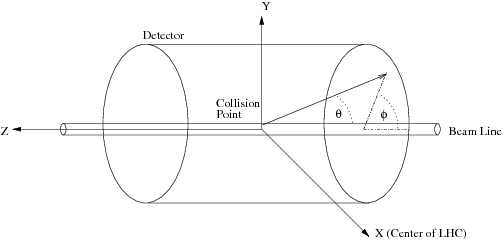
\includegraphics[width=0.65\textwidth]{../figs/Exp/CMScoord.png}}
%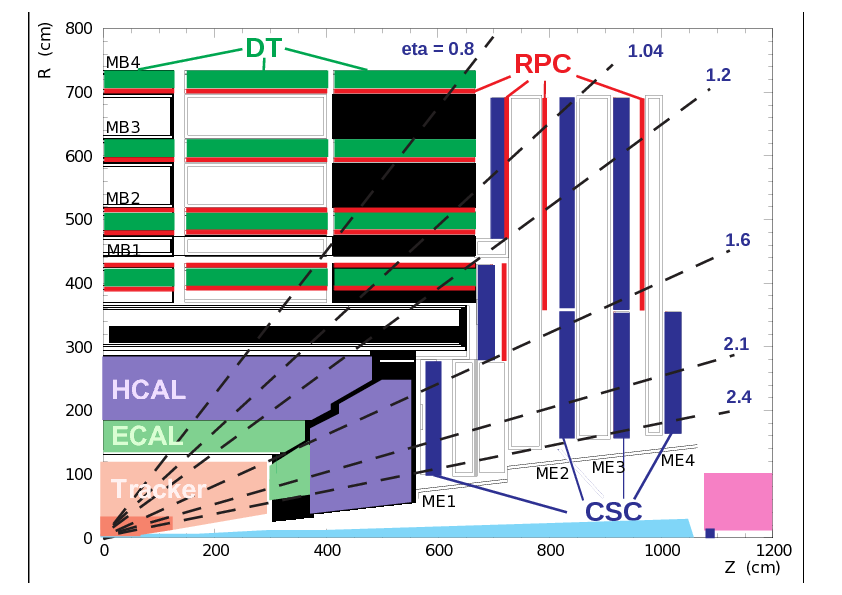
\includegraphics[width=0.45\textwidth]{../figs/Exp/CMScoord_eta.png}}
    \caption{CMS coordinate system. }
    \label{fig:CMScoord}
  \end{center}
\end{figure}

\begin{figure}[htb]
  \begin{center}
    {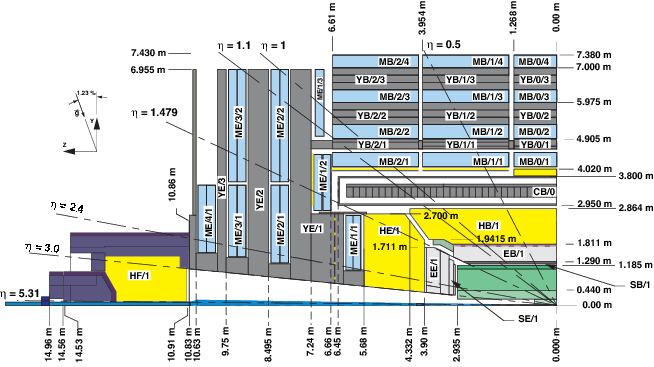
\includegraphics[width=0.98\textwidth]{../figs/Exp/CMSview1.png}\\
     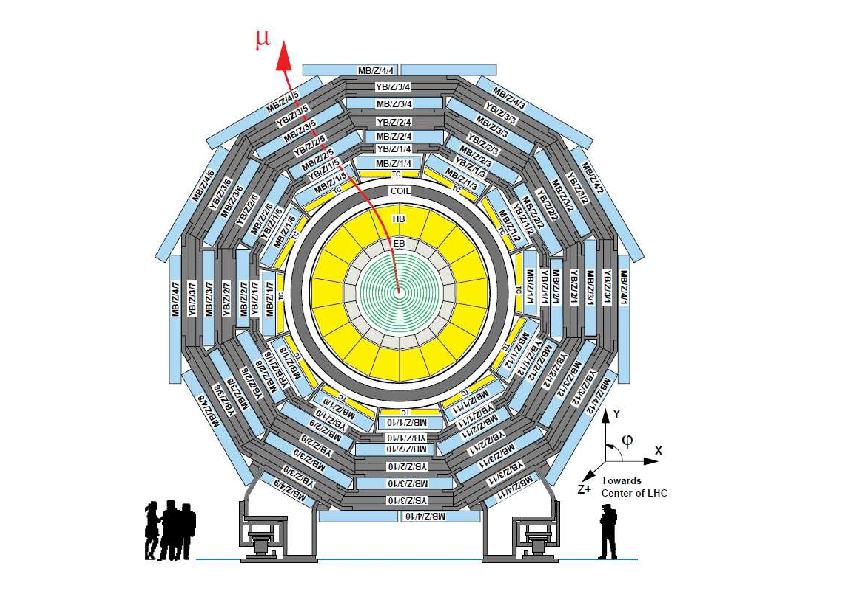
\includegraphics[width=0.98\textwidth]{../figs/Exp/CMSview.png}}
    \caption{CMS detector, schematic view. Top: $r-z$ plane, bottom: $r-\phi$ plane at $z=0$~\cite{ref_CMSschemView}. The tracking system is shown in green, EB and EE of ECal are shown in gray, HB, HE and HF of HCal are shown in yellow. HCal is surrounded by a magnet which is shown in gray and white. Muon stations and return yokes are located outside of the magnet and are shown in blue and gray. A red line at the bottom plot is a muon trajectory demonstrating that a typical muon penetrates through the whole CMS detector. People at the bottom illustrate the scale of the CMS detector.}
    \label{fig:CMSschemView}
  \end{center}
\end{figure}

The detector consists, from the inner to the outer layer,  of a tracking system, an electromagnetic calorimeter (ECal), a hadronic calorimeter (HCal), a magnet and a muon system. A slice of CMS in the $r$-$\phi$ plane is shown in Fig.~\ref{fig:CMS_slice}.

Most heavy particles produced in a collision decay immediately, and we detect their long-lived decay products including electrons, photons, muons, neutral or charged hadrons. Particles which can be detected by CMS are referred as ``visible'' particles in contrast to ``invisible'' particles which cannot be detected by CMS because their probabilities to interact with any part of the detector are very low. The SM example of an invisible particle is a neutrino.

We can identify the type of particle by the trace it leaves in different subdetectors. Charged particles interact with the substance of the tracking system which performs several position measurements of the particles. The sequence of these position measurements is called a track. Neutral particles do not leave any trace in the tracking system because they do not ionize atoms. 

Thus, electrons and positrons leave tracks in the tracking system while photons do not. Both these types of particles induce showers in the ECal of the same shapes, and are distinguished by having or not having a spatially matching track. Hadrons normally travel through the ECal undisturbed and induce a hadronic shower in the HCal (Ch.~\ref{sec:Exp_CMS_HCal}). Charged and neutral hadrons are distinguished from each other by linking or not linking to the tracks, similarly to how electrons are distinguished from photons. Muons are the only particles which penetrate through the ECal, the HCal and the magnet and leave tracks in the CMS muon system. Neutrinos are not directly detected by CMS.   

\clearpage

\begin{figure}[htb]
  \begin{center}
    {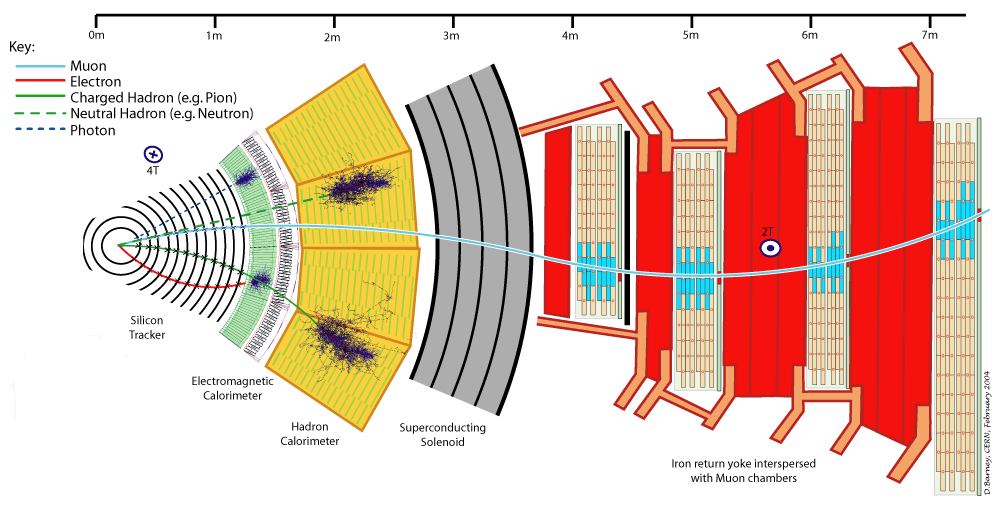
\includegraphics[width=0.98\textwidth]{../figs/Exp/CMS_Slice.png}}
    \caption{CMS detector, a schematic view of a segment in the $r$-$\phi$ plane at $z=0$. Traces left by muons, electrons, photons, charged and neutral hadrons in different subdetectors are shown.}
    \label{fig:CMS_slice}
  \end{center}
\end{figure}

All subdetectors are essential for the $W\gamma$ measurement, and the remainder of this chapter describes the subdetectors in greater detail. Muons and electrons, which we have as final state particles in the $W\gamma$ measurement, are both affected by the CMS magnetic field, allowing the tracking system and the muon system to measure their trajectory parameters and momenta. In this dissertation we use the information of the primary vertex, the collision point, determined by the tracking system, to select our events. The tracking system also provides us information about electron and muon trajectories and momenta and is used for distinguishing between electrons and photons. The ECal is necessary to identify electrons and photons and to measure all kinematic parameters of photons. The HCal is also used for electron and photon identification: the energy deposit in the HCal left by an electron or a photon must be very small compared to the energy deposit left in the ECal. The muon system is essential for muon reconstruction and identification.

\clearpage

\subsection{Magnet}
% CONTENT-WISE IS OK

A magnetic field in a particle detector is necessary to measure momenta of charged particles by track curvatures. The higher the momentum is, the less a particle trajectory is affected by the magnetic field. In the plane, transverse to the beamline, this relation is:
\begin{equation}
  R=\frac{P_T}{qB},
\end{equation} 
\noindent{where $R$ is a radius of a projection of a charged particle's trajectory to the transverse plane, $P_T$ and $q$ are the particle's transverse momentum and electric charge, and $B$ is the magnetic field. In CMS, the tracking system measures  momenta of all charged particles. Also, the muon system measures momenta of muons. }

The CMS magnet is placed between the HCal and the muon system. The magnet is made of superconducting wires that are cooled to~$-268.5^0$C by a cryogenic system based on a liquid helium flow~\cite{ref_MagnetCryo}. An electric current flowing in the wires creates a uniform field of $B=4$T inside the solenoid, for the tracking system, and also provides a smaller magnetic field of a certain configuration outside the solenoid, for the muon system. The stronger field in the tracking system is necessary because of higher track density and smaller size relative to the muon system.

\subsection{Tracking System}
%"The tracker is designed in such a way that a single track hits multiple sensors."
%    "Then the trajectory is reconstructed based on how much charge is collected on each sensor."
%       What does it mean, exactly, each of these sentences? It is not clear to me.

The tracking system measures parameters of particle trajectories, locations of primary and secondary vertices, and momenta of charged particles. It is designed to disturb particle as little as possible when they pass through to be able to accurately measure its energy deposit in ECal or HCal or, in case of a muon, accurately reconstruct a track in the muon system. The goals of little disturtion in the tracking system and high pecision track reconstruction at the same time are achived by CMS algorithms being capable of reconstructing a trajectory with just a few position measurements (``hits''), each as accurate as~$\sim10~\mu$m in the transverse plane and~$\sim30~\mu$m in the longitudinal direction~\cite{ref_trackerPerformance}.

Tracks that originate from proton collisions, collision tracks, start at the center and then cross the layers of the tracking system. Charged particles take helical paths in the magnetic field. Tracks are straight in the $r-z$ plane and curved by the magnetic field in the $r$-$\phi$ plane. The acceptance of the tracker system in the $r$-$z$ plane is geometrically limited by the absolute value of the pseudorapidity $|\eta| \leq 2.5$.

The tracking system consists of silicon pixels and silicon strips (Fig.~\ref{fig:tracker_slice}). The pixel tracker is the closest subsystem of CMS to the collision point. Thus it experiences the largest particle flux: at~8~cm from the collision point the flux is about~10~million/(cm$^2$s), and the pixel detector with its~65~million pixels is capable of reconstructing all these tracks. It consists of three cylindrical layers of pixel sensors in the barrel with radii of~4~cm,~7~cm and~11~cm which are referred as barrel pixel subdetectors (BPIX) and four disks in the endcap, two disks at each side, which are referred as forward pixel subdetector (FPIX). Pixel modules provide 3D position measurements as well as some of the stpip modules while the other strip modules provide 2D position measurements.

%The tracker is designed in such a way that a single track hits multiple sensors. Then the trajectory is reconstructed based on how much charge is collected on each sensor. This allows us to reach a spacial resolution of~15-20~$\mu$m which is much smaller than a distance between sensors.

The strip tracker is placed right outside the pixel tracker and occupies the detector volume up to~130~cm from the beam axis. The strip tracker consists of four parts: the tracker inner barrel (TIB), the tracker inner disks (TID), the tracker outer barrel (TOB) and the tracker endcap (TEC) as shown in Fig.~\ref{fig:tracker_slice}. %In the strip tracker, there are over~15,000 sensitive modules with a total number of~10~million strips. Each sensitive module consists of a set of sensors, its support structure, and readout elements.

The resolution of track parameters depends on a type of the reconstructed particle, its transverse momentum and pseudorapidity. For example, a momentum resolution of an isolated muon with $P_T^{\mu}=100~$GeV and $\eta^{\mu}=0$ is~2\% and increases with $|\eta|$ as shown in~\cite{ref_trackerPerformance}, Fig.~14.  

%electric charge and amplification

%limitations

%QUOTE:
%Knowing which pixels have been touched allows us to deduce the particle's trajectory. And because the detector is made of 2D tiles, rather than strips, and has a number of layers, we can create a three-dimensional picture.

\begin{figure}[htb]
  \begin{center}
    {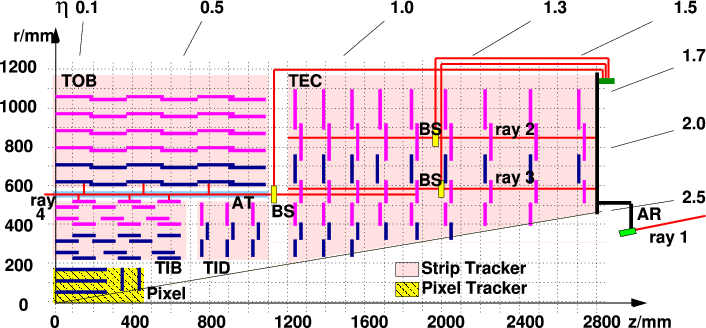
\includegraphics[width=0.8\textwidth]{../figs/Exp/tracker_slice.png}}
    \caption{Slice of the CMS tracking system in the $r$-$z$ plane. Pixel modules and strip modules shown in blue provide 3D position measurements. Strip modules shown in pink provide 2D position measurements. }
    \label{fig:tracker_slice}
  \end{center}
\end{figure}

\subsection{Electromagnetic Calorimeter}

The ECal is placed between the tracking system and the HCal. It is made of high-density lead tungstate crystals arranged in a barrel section and two endcap sections. The crystals are scintillators. When electrons and photons pass through the scintillators, they produce light proportional to the particle's energy. The scintillated light is then amplified by photomultipliers. After that, signals are digitized and taken away by fiber optic cables.

The ECal measures the energy of electrons and photons and parameters of their trajectories. In order to distinguish between electrons and photons, it is necessary to perform spatial matching to the track in the tracking system. If there is a track, then the particle is an electron (or positron), otherwise the particle is a photon.

It is important for the ECal to be able to distinguish between a single energy photons of high energy and pairs of almost collinear photons of lower energy e.g. from a $\pi^0$ decay. It is especially difficult in the endcap sections where the angle between two photon trajectories is small. It is achieved with ECal preshower detectors (PS) which have~$\sim$15~times smaller granularity are located in front of the endcaps. Such a small granularity is achived by making preshower of two lead planes a followed by silicon sensors rather than of lead crystals followed by photomultipliers. The ECal PS provide extra spatial precision. 

The ECal energy resolution depends on photon or electron energy and of the ECal pseudorapidity region. The resolution is 2\%-5\% for electrons from $Z\rightarrow ee$, and 1\%-5\% for photons from $H\rightarrow\gamma\gamma$~\cite{ref_ECalResolution}.

%Their strips are~2~mm wide compared to~3~cm wide crystals in the main volume of the ECal.

%(Why muons and hadrons don't release their energy here?)
%limitations

\subsection{Hadron Calorimeter}
\label{sec:Exp_CMS_HCal}
The HCal measures the energy of charged and neutral hadrons. It consists of the barrel, endcap and forward parts: HB, HE and HF in Fig.~\ref{fig:CMSschemView}, top, respectively. HCal is designed to stop all hadrons passing through, thus, it extends to $|\eta|=5.3$ for forward HCal.

The HCal is a sampling calorimeter. It consists of alternating layers of brass and steel bsorbers and plastic scintillators. When a hadron hits an absorber, it induces a hadronic shower. The light produced by the shower is collected on optic fibers and passed to the readout system. The total amount of light released in a certain region of the HCal is a measure of hadron's energy. In addition to the energy, the HCal also reconstructs the trajectory of the hadron.   

\subsection{Muon System}

%(1) QUOTE
%Because muons can penetrate several metres of iron without interacting, unlike most particles they are not stopped by any of CMS's calorimeters. Therefore, chambers to detect muons are placed at the very edge of the experiment where they are the only particles likely to register a signal.
%(1) MY WORDS
Muons, unlike other visible particles, are not stopped by CMS calorimeters because they neither induce an electromagnetic shower in the ECal nor a hadronic shower in the HCal. The muon system, which is placed outside the magnet and which is the largest by spatial size part of the CMS detector, is designed to register muons.

There are four concentric layers of muon detectors (stations) and the iron return yoke between them. Muons induce several hits in the muon stations which are later fitted and matched to the tracking system measurements to provide the best possible resolution in the measurements of the muon's trajectory and momentum.

There are three types of muon chambers used in the CMS muon system: drift tubes (DTs), cathode strip chambers (CSCs) and resistive plate chambers (RPCs) (Fig.~\ref{fig:muonSystem}). Overall, there are~1400~muon chambers including~250~DTs,~540~CSCs and~610~RPCs.

%DTs
%(4) QUOTE:
%The drift tube (DT) system measures muon positions in the barrel part of the detector. Each 4-cm-wide tube contains a stretched wire within a gas volume. When a muon or any charged particle passes through the volume it knocks electrons off the atoms of the gas. These follow the electric field ending up at the positively-charged wire.
%By registering where along the wire electrons hit (in the diagram, the wires are going into the page) as well as by calculating the muon's original distance away from the wire (shown here as horizontal distance and calculated by multiplying the speed of an electron in the tube by the time taken) DTs give two coordinates for the muon’s position.
%Each DT chamber, on average 2m x 2.5m in size, consists of 12 aluminum layers, arranged in three groups of four, each up with up to 60 tubes: the middle group measures the coordinate along the direction parallel to the beam and the two outside groups measure the perpendicular coordinate.
%(4) MY WORDS:
The system of DTs measures positions of muons in the barrel. Each DT chamber is about~2~m by~2.5~m in size. A chamber consists of~12~layers of aluminum which are arranged in groups of four. There are up to~60~DTs in a layer. The middle group of layers measures $z$-coordinate and two other groups determine the perpendicular coordinate. The DT's volume is filled with a gas, and there is a wire inside. When a charged particle passes through the volume, it ionizes atoms. Released electrons drift in the electric field to the positively-charged wire. The position along the wire is registered, and the distance of the muon away from the wire is calculated providing measurements of two coordinates of the position of the muon.

%CSCs
%(5) QUOTE:
%Cathode strip chambers (CSC) are used in the endcap disks where the magnetic field is uneven and particle rates are high.
%CSCs consist of arrays of positively-charged “anode” wires crossed with negatively-charged copper “cathode” strips within a gas volume. When muons pass through, they knock electrons off the gas atoms, which flock to the anode wires creating an avalanche of electrons. Positive ions move away from the wire and towards the copper cathode, also inducing a charge pulse in the strips, at right angles to the wire direction.
%Because the strips and the wires are perpendicular, we get two position coordinates for each passing particle.
%In addition to providing precise space and time information, the closely spaced wires make the CSCs fast detectors suitable for triggering. Each CSC module contains six layers making it able to accurately identify muons and match their tracks to those in the tracker.
%(5) MY WORDS

CSCs are placed in the endcap regions. CSCs are arrays of anode wires crossed by copper cathode strips placed in a gas volume. When a charged particle penetrates the gas volume, it ionizes the gas. Electrons drift to the wires while ions move to the strips, and charge pulses are induced on wires as well as on strips. Strips are perpendicular to wires. Thus we measure two coordinates for each particle.  

% RPCs
%(6) QUOTE:
%Resistive plate chambers (RPC) are fast gaseous detectors that provide a muon trigger system parallel with those of the DTs and CSCs. RPCs consist of two parallel plates, a positively-charged anode and a negatively-charged cathode, both made of a very high resistivity plastic material and separated by a gas volume.
%When a muon passes through the chamber, electrons are knocked out of gas atoms. These electrons in turn hit other atoms causing an avalanche of electrons. The electrodes are transparent to the signal (the electrons), which are instead picked up by external metallic strips after a small but precise time delay. The pattern of hit strips gives a quick measure of the muon momentum, which is then used by the trigger to make immediate decisions about whether the data are worth keeping. RPCs combine a good spatial resolution with a time resolution of just one nanosecond (one billionth of a second).
%(6) MY WORDS: 
RPCs are parallel capacitors made of high-resistivity plastic plates with a space between them filled with gas. RPCs provide quick measurements of muon momenta. A muon passing through the RPC ionizes gas atoms. Released electrons ionize more atoms inducing an avalanche in the electric field. Electrodes receive signal and pass it to external strips that provide a quick measurement of the muon's position which is subsequently transformed to the momentum measurement by the trigger's electronics. 


\begin{figure}[htb]
  \begin{center}
    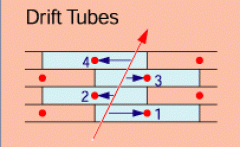
\includegraphics[height=2.5 cm]{../figs/Exp/muonSystem_driftTubes.png}\quad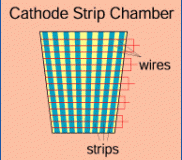
\includegraphics[height=2.5 cm]{../figs/Exp/muonSystem_CSC.png}\quad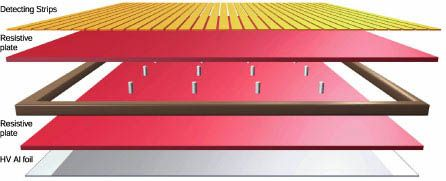
\includegraphics[height=2.5 cm]{../figs/Exp/muonSystem_RPC.png}
    \caption{Components of the CMS muon system. Left to right: drift tubes (DTs), cathode strip chambers (CSCs), resistive plate chambers (RPCs).}
    \label{fig:muonSystem}
  \end{center}
\end{figure}


\subsection{Triggering and Data Acquisition}

At peak luminosity, CMS experiences~40~million proton-proton collisions per second that come in bunches separated by~25~ns. It is not technically feasible to read out all these events. Moreover, we do not need most of these events for a physics measurement because most of them have not resulted from an interesting physics process. We have resources to store about one hundred events out of forty million, and that is why we need a trigger system that quickly decides what the best one hundred events are.

%New events come before the events from the previous bunch crossing left the detector. To process the information from many different collisions at the same time, data is stored in pipelines.

If the triggers were not strict enough, and we would select one hundred events too quickly, e.g., in~1/10~s, then CMS would not be able to process the remaining~90\% of events provided by LHC in a given second and we would lose~90\% of potentially interesting events.

If the triggers were too strict, we would select, e.g.,~ten events per second, not one hundred and lose CMS's potential to store and process data by~90\% which would significantly reduce our chances for discovery and increase statistical uncertainties for precision measurements.

Thus, the challenge of the trigger system is to select the best one hundred events per second and do so quickly to be able to process every single event. To achieve this goal, a two-level trigger system was developed consisting of the Level~1 trigger (L1T) and the High Level Trigger (HLT) as shown in Fig.~\ref{fig:trigger_2level}.

L1T is a hardware based trigger (Fig.~\ref{fig:trigger_L1}). It uses information from the ECal, HCal and muon system. L1T reduces the frequency of coming events from~40~MHz to~100~kHz. Events that did not pass the L1T are lost forever while events that pass the L1T are temporarily stored to be checked by the HLT.

HLT is a software-based trigger. It uses information from all subdetectors and runs fast reconstruction and identification algorithms to determine types of particles and their kinematics. It reduces the event rate to~100~Hz. Events that did not pass HLT are lost forever. Events that pass HLT are arranged into appropriate datasets depending on HLT selection criteria they passed and stored for physics measurements.

\begin{figure}[htb]
  \begin{center}
    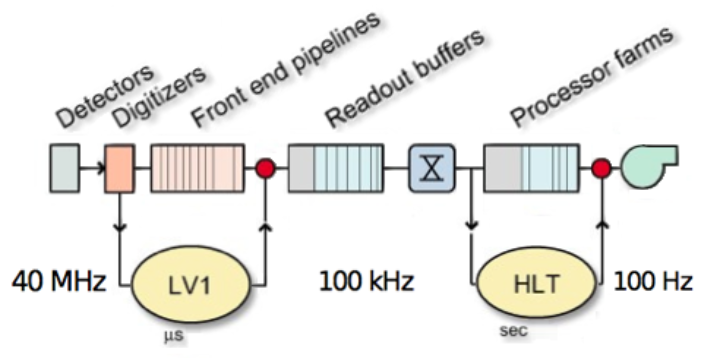
\includegraphics[width=0.8\textwidth]{../figs/Exp/trigger_2level.png}
    \caption{Two-level CMS trigger system.}
    \label{fig:trigger_2level}
  \end{center}
\end{figure}

\begin{figure}[htb]
  \begin{center}
    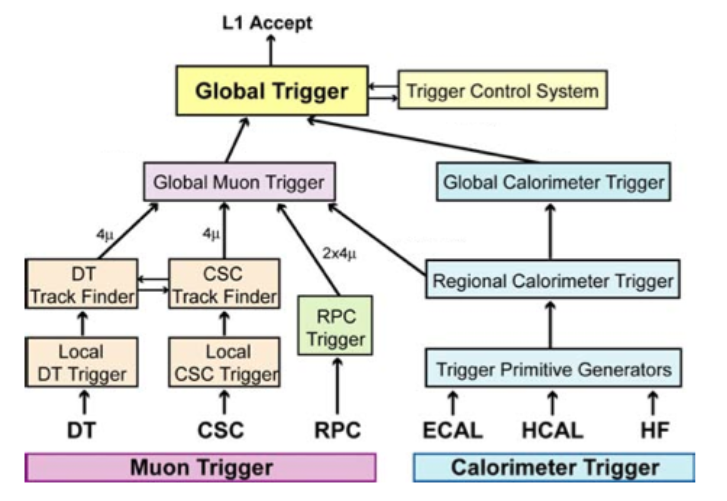
\includegraphics[width=0.8\textwidth]{../figs/Exp/trigger_L1.png}
    \caption{Level~1 CMS trigger system.}
    \label{fig:trigger_L1}
  \end{center}
\end{figure}

\subsection{Particle Flow Algorithm of Event Reconstruction}

A particle flow (PF) algorithm is used by CMS to identify and reconstruct stable particles~\cite{ref_ParticleFlowAlg}. It processes the information from all CMS subdetectors and identifies and reconstructs each stable particle in an event individually. The list of particles include muons, electrons, photons, charged and neutral hadrons. Each type of particles leaves its specific trace in the CMS detector as shown in Fig.~\ref{fig:CMS_slice}. After reconstruction of individual stable particles, jets are built, missing transverse energy $E_T^{miss}$ is determined, certain short-lived particles are reconstructed based on the list of individual stable particles in the event.

One particle can induce several different particle-flow elements in different subdetectors. The linking algorithm links these elements together producing blocks of elements. Usually, a block has between one and three elements. Links can be connections between the tracking system and PS, ECal or HCal, between PS and ECal, between ECal and HCal, and between a tracking system and a muon system. 

In each block, muons are considered first. A link between charged tracks in the tracking and muon systems comprise a global muon which produces one ``particle-flow muon''. The corresponding track in the tracking system is removed from the block and corresponding energy deposits are subtracted from ECal and HCal. Then electrons are reconstructed and identified using the tracking system and ECal. The corresponding tracks and ECal clusters are removed from the block. Remaining tracks and clusters are considered more carefully to identify charged hadrons, neutral hadrons, and photons.

When all particles in the event are reconstructed and identified, the algorithm determines missing transverse energy $E_T^{miss}$ as 
\begin{equation}\label{eq:MET}
  E_T^{miss} = - | \sum \mathbf{P_T} |,
\end{equation}
\noindent{where the summation covers all visible particles in the event. For precise measurement of $E_T^{miss}$ it is important to capture the full energy release of all visible particles.}

$E_T^{miss}$ is used in physics measurements as a measure of $P_T$ of neutrinos and other invisible particles in the event. Fake $E_T^{miss}$ can originate from particles that did not fall into the detector acceptance, particles that they did not reach the tracking system because their momenta was too low and, therefore, track curvature was too high, momenta mismeasurement, particle misidentification, cosmic rays particles, and machine background.

In the measurement of this dissertation PF muons, electrons, photons, and $E_T^{miss}$ are used for all the major steps of the cross section measurement including event selection, background subtraction, various corrections, and determination of phase space restrictions and bin boundaries. Each step is described in greater details in~Ch.~\ref{sec:AN_WgMeas}. 

%Acceptance: particles which are too collinear and go to pipe; particles which get curved too strongly
